%% main.tex -- IEEE T-BIOM submission (regular paper).
%% Target: IEEE Transactions on Biometrics, Behavior, and Identity Science.
%% Compile: pdflatex main ; bibtex main ; pdflatex main ; pdflatex main
\documentclass[journal]{IEEEtran}

% --- packages ---
\usepackage[T1]{fontenc}
\usepackage[utf8]{inputenc}
\usepackage{cite}
\usepackage{graphicx}
\graphicspath{{../../../shared/figures/}}
\usepackage{amsmath,amssymb,amsfonts}
\usepackage{textcomp}
\usepackage{array}
\usepackage{booktabs}
\usepackage{enumitem}
\usepackage{url}
\usepackage{xcolor}
\usepackage{microtype}
\setlength{\emergencystretch}{2em}

% RED: real data the authors must still supply before submission.
\newcommand{\fillin}[1]{\textcolor{red}{\textbf{[#1]}}}

\begin{document}

\title{Cross-Age Face Verification from Mined Same-Person Social-Media Pairs:\\ A Naturally-Supervised Longitudinal Signal}

\author{Danil~F.~Volkhin and Ivan~S.~Kopylov%
\thanks{Manuscript prepared in 2026.}%
\thanks{D.~F.~Volkhin (author) and I.~S.~Kopylov (scientific advisor) are with the National Research University Higher School of Economics (HSE University), Moscow, Russia (e-mail:~deneal123@mail.ru; ORCID:~0009-0000-8108-8814).}%
\thanks{Non-sensitive code, configurations and aggregate statistics are available at \texttt{https://github.com/deneal123/ChildVSAdult}; no faces, biometric templates or row-level private-corpus protocol are released.}}

\markboth{IEEE Transactions on Biometrics, Behavior, and Identity Science,~Vol.~XX, No.~X, Month~Year}%
{Volkhin \MakeLowercase{\textit{et al.}}: Cross-Age Face Verification from Mined Same-Person Social-Media Pairs}

\IEEEtitleabstractindextext{%
\begin{abstract}
Cross-age face verification lacks longitudinal training data. We mine weak same-person pairs from social-media ``then/now'' posts using caption parsing and embedding-based person clustering, without manual identity or age labels. On an endpoint-age-matched FG-NET protocol, fine-tuning FaceNet raises large-gap ($\geq$25-year) ROC-AUC from \textbf{0.802 to $0.8490\pm0.0016$} across three seeds; the mean gain is $+0.0467\pm0.0016$, with positive paired subject-bootstrap 95\% intervals on the same subjects. The larger $+0.112$ gain from the original random-impostor protocol is not the corrected headline. LFW improves slightly, CALFW/CACD-VS AUC is unchanged, and AgeDB-30 decreases by 0.008; an internal endpoint-matched test gains AUC but loses low-FAR TAR. A strong AdaFace IR-101 recognizer drops from 0.961 to 0.376 ROC-AUC when impostors are look-alikes instead of random. Contrastive and ArcFace-margin objectives perform similarly under the original protocol, and a fixed-step within-VK control favors large-gap over short-gap training pairs by $+0.0257\pm0.0009$ AUC. This is not a causal source effect: age/quality covariates, generic-face controls and identity-overlap adjudication remain unresolved. Bidirectional VK--Reddit transfer and a gap-parity re-aging control provide bounded external evidence.
\end{abstract}

\begin{IEEEkeywords}
Cross-age face recognition, age-invariant representation, naturally/weakly-supervised identity, dataset curation, shortcut learning, fairness, calibration.
\end{IEEEkeywords}}

\maketitle
\IEEEdisplaynontitleabstractindextext
\IEEEpeerreviewmaketitle

\section{Introduction}\label{sec:intro}
\IEEEPARstart{C}{ross-age} face verification arises in archival retrieval, account recovery, and authorized search for missing persons. The challenge lies not in discriminating among arbitrary individuals but in distinguishing \emph{the same person across age} from \emph{different people of similar age and appearance}. Annotating longitudinal identity pairs (one individual across many years) is costly, and such data remain scarce, which constrains supervised approaches; recent work continues to identify both the shortage of cross-age supervision and cross-dataset generalization as central problems~\cite{wang2024cacon,cao2026hmlf}.

\textbf{Hypothesis.} A multi-photo ``then/now'' post showing one person at different ages yields $\binom{n}{2}$ positive identity pairs without manual annotation; a caption stating ages adds a secondary age anchor. The same-person pairing is the operative signal (an ablation later isolates the age anchor at a marginal $+$0.009); this is a scalable, naturally-supervised signal of cross-age identity, and fine-tuning a weak recognizer on it should transfer to external benchmarks.

\textbf{Contributions (bounded).}
(1)~A weakly/naturally-supervised (no manual id/age labels) longitudinal signal mined from social posts---same-person identity pairs, with caption age anchors only a secondary cue.
(2)~A reproducible curation pipeline with component audits, quality/sensitivity analysis, and the finding that naive positive counts are inflated about $2\times$ by near-duplicate frames.
(3)~A rigorous \emph{attribution protocol} (one weak trainable backbone, frozen vs.\ fine-tuned, external evaluation) isolating the contribution of \emph{data} from network capacity.
(4)~A bounded account of where the gain does and does not persist: comparisons across tested objectives, backbones, source communities and external benchmarks, plus explicit low-FAR trade-offs. The effect of longitudinal pairing relative to matched-source controls remains to be established.

We emphasize that the novelty is data-centric rather than architectural---a new \emph{origin of supervision}---and should be evaluated accordingly.

\section{Related Work and Positioning}\label{sec:related}
\noindent\textbf{Age disentanglement and synthesis.}
OE-CNN (orthogonal embedding decomposition)~\cite{wang2018oecnn}, DAL (decorrelated adversarial
learning)~\cite{wang2019dal}, MTLFace (recognition, age synthesis and attention decomposition)~\cite{huang2021mtlface},
and CDD-AFL (class-wise domain decoupling with adversarial feature learning)~\cite{wu2024cddafl}
learn age-invariant features from manually labeled identity/age data. Face-aging augmentation is a
second route, but controlled studies find only partial recognition gains~\cite{yao2024synthageing}.

\noindent\textbf{Contrastive and data-centric supervision.}
CACon adds a synthesized cross-age view to a multi-positive contrastive objective~\cite{wang2024cacon};
OrdCon explicitly models ordinal age progression for cross-dataset generalization~\cite{wang2025ordcon}.
HMLF combines margin and contrastive losses without age labels for \emph{1:N retrieval}~\cite{cao2026hmlf};
its mAP/Rank-$k$ protocol is complementary, not a 1:1 verification baseline. Generic SimCLR-style
augmentation~\cite{chen2020simclr} lacks identity anchors across time. We instead mine the structure
``one post $=$ one person at different ages'' as a naturally-supervised positive-pair generator.

\noindent\textbf{Scope and evaluation.}
Direct cross-age methods above are separated from LARNet/LARNeXt, which model a \emph{pose}-induced
feature residual~\cite{yang2021larnet,yang2023larnext} and motivate our diagnostics only by analogy.
The standard evaluation datasets---CACD~\cite{chen2014cacd}, MORPH~\cite{ricanek2006morph},
AgeDB~\cite{moschoglou2017agedb}, FG-NET~\cite{panis2016fgnet}, and CALFW~\cite{zheng2017calfw}---mix
verification, identification, and retrieval protocols, so published headline numbers cannot establish
controlled superiority. Table~\ref{tab:positioning} positions the supervision mechanisms; the supplement
separates published-number comparisons from our common-protocol reproductions.

\begin{table*}[!t]
\renewcommand{\arraystretch}{1.25}
\caption{Positioning vs.\ Prior Work.}
\label{tab:positioning}
\centering
\footnotesize
\begin{tabular}{@{}p{0.16\textwidth}p{0.16\textwidth}p{0.30\textwidth}p{0.30\textwidth}@{}}
\toprule
Work & Supervision & Mechanism & Our difference \\
\midrule
OE-CNN (2018)~\cite{wang2018oecnn} & labeled id$+$age & orthogonal feature decomposition & no manual id/age labels, not decomposition \\
DAL (2019)~\cite{wang2019dal} & labeled id$+$age & adversarial id/age factorization & mined pairs $+$ simpler objective \\
MTLFace (2021)~\cite{huang2021mtlface} & labeled id$+$age & recognition $+$ age synthesis (multi-task) & weaker pipeline; novel supervision origin \\
CACon (2024)~\cite{wang2024cacon} & semi-sup.\ $+$ synthetic & contrastive on synthesized cross-age & natural cross-time views; controlled reproduction \\
Synthetic Ageing (2024)~\cite{yao2024synthageing} & synthetic & train on aged images & we make \emph{real} mining the thesis \\
OrdCon (2025)~\cite{wang2025ordcon} & age-ordered contrastive & order-enhanced features & mine natural pairs, no explicit age order \\
\bottomrule
\end{tabular}
\end{table*}

We report the canonical verification suite (AgeDB-30, CALFW, CACD-VS and FG-NET; CALFW is an
age-gapped LFW protocol~\cite{huang2007lfw}). The goal is \emph{not} absolute leaderboard superiority:
we use a weak backbone for clean attribution and quantify the transfer from a naturally-supervised
source; Sec.~\ref{sec:res-objective} then compares complete methods under one controlled protocol.

\section{Data: Naturally-Anchored Longitudinal Pairs}\label{sec:data}
\textbf{Source.} Two public ``then/now'' multi-photo communities on VK (one platform, Russian-language context). Faces are detected and aligned with a 5-point ArcFace template (InsightFace RetinaFace~\cite{deng2020retinaface}, \texttt{buffalo\_l}). A \emph{usable} face passes detection-score, minimum-size, blur, and single-target checks. Figure~\ref{fig:pipeline} makes the full sequence, thresholds and measured yield explicit; Table~\ref{tab:scale} separates raw photos from processed face records.

\begin{figure*}[!t]
\centering
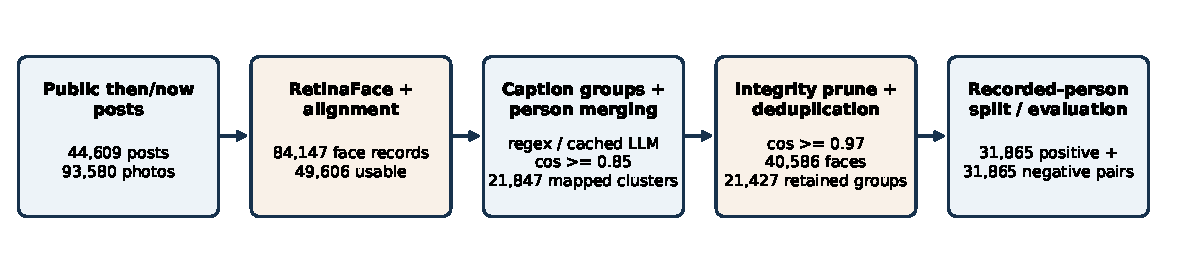
\includegraphics[width=\textwidth]{fig_pipeline.pdf}
\caption{End-to-end data and evaluation pipeline. Automatic caption/integrity decisions are versioned and cached; the prepared held-out audit contains 400 blinded items for each of five targets and requires two independent annotators plus adjudication. No audit item is used to tune the clustering (0.85) or near-duplicate (0.97) threshold. Counts are generated from the machine-readable funnel artifact.}
\label{fig:pipeline}
\end{figure*}

\begin{table*}[!t]
\renewcommand{\arraystretch}{1.2}
\caption{Dataset Scale (Raw Mined) and After Curation (Sec.~\ref{sec:data-curation}).}
\label{tab:scale}
\centering
\footnotesize
\begin{tabular}{@{}lrrrrrr@{}}
\toprule
Stage & Posts & Photos & Face records & Usable faces & Persons & Positives \\
\midrule
Raw mined (2 communities) & 44{,}609 & 93{,}580 & 84{,}147 & 49{,}606 & 21{,}847 & 65{,}897 \\
\textbf{After curation} & --- & --- & --- & \textbf{40{,}586} & \textbf{21{,}427} & \textbf{31{,}865} \\
\bottomrule
\end{tabular}
\end{table*}

\subsection{Age Extraction}\label{sec:data-age}
Captions are parsed by regular expressions (Russian patterns plus the slash format ``6/18/21'', one age per photo) and GigaChat-2-Max, a Russian-oriented LLM family~\cite{gigachat2025family}. The frozen run uses temperature $10^{-5}$, top-$p=0$, a hashed prompt and cached responses. The model was selected for Russian-language support, not brand recognition; a final quality justification is conditional on the prepared human-gold comparison against regex and a reproducible local model. Recomputing the comparison directly from all 33{,}697 cached multi-photo captions (Table~\ref{tab:age}) gives 78.1\% exact agreement (including both-empty outputs); 15.5\% return different non-empty age sets, while LLM-only and regex-only outputs account for 3.4\% and 3.0\%. These figures are an automatic cross-check, not accuracy against human ground truth. We do not treat either system as ground truth: a preregistered multi-annotator audit is required before resubmission, and downstream explicit age anchors contribute only marginally (Sec.~\ref{sec:res-main}).

\begin{table}[!t]
\renewcommand{\arraystretch}{1.2}
\caption{Age-Extraction Audit: LLM vs.\ Regex (33{,}697 Captioned Multi-Photo Posts).}
\label{tab:age}
\centering
\footnotesize
\begin{tabular}{@{}lrr@{}}
\toprule
Category & $n$ & Share \\
\midrule
Agree (same ages or both empty) & 26{,}312 & 78.1\% \\
LLM-only ages & 1{,}162 & 3.4\% \\
Different non-empty ages & 5{,}207 & 15.5\% \\
Regex-only ages & 1{,}016 & 3.0\% \\
\bottomrule
\end{tabular}
\end{table}

\subsection{Persons and Leakage-Safe Split}\label{sec:data-persons}
A naive ``one post $=$ one identity'' undercounts: a person recurs across posts. Each usable crop is embedded by InsightFace ArcFace R50 \texttt{w600k\_r50}; post-groups are graph nodes, an edge is added when any cross-group face pair has cosine $\geq0.85$, and union--find connected components define a \emph{person}. This gives 21{,}848 persons from 27{,}487 post-groups ($\approx$20\% recurrence), which are split \emph{by person} (not by post). We deliberately exclude the ambiguous lower-similarity band rather than infer identity from it. An independent FaceNet/CASIA sweep yields 21{,}484 persons at the same threshold (1.7\% difference) and preserves the 52\% near-duplicate reduction; the blinded boundary audit remains required before resubmission.

\subsection{Auditing the Automatic Supervision}\label{sec:data-audit}
The automatic supervision components are potential hidden label noise. Current corpus-scale checks are LLM-vs-regex age agreement (Table~\ref{tab:age}), conservative high-cosine person clustering, group-integrity classification, and deduplication sensitivity. As an additional noise proxy, InsightFace \texttt{buffalo\_l/genderage.onnx} assigns an apparent binary gender per usable crop; a group's consistency is the fraction agreeing with its majority label, and 2{,}919 multi-photo groups below 0.6 are flagged rather than silently treated as reliable. Ties/low-consistency groups remain uncertain, and this estimator is neither self-identified gender nor identity evidence. These checks characterize internal consistency but are \emph{not} human ground truth. A preregistered audit with two independent annotators, held-out samples, agreement coefficients and confidence intervals is required before resubmission; until it is completed, the paper makes no quantitative claim of human-validated label precision.

\subsection{Curation Pipeline and Its Largest Finding}\label{sec:data-curation}
Three steps: (i)~\emph{apparent gender/age metadata} (estimator) per face, aggregated per person---the corpus is 76.7\% apparent-female / 23.3\% apparent-male; (ii)~\emph{LLM group-integrity validation} (Table~\ref{tab:integrity})---person-clustering had already separated most multi-person posts, so only 421 person-groups are flagged noisy; (iii)~\emph{near-duplicate dedup} within each person (cosine $\geq$ 0.97), removing 8{,}190 faces ($\approx$17\%).

\begin{table}[!t]
\renewcommand{\arraystretch}{1.2}
\caption{LLM Group-Integrity Classification (33{,}697 Posts).}
\label{tab:integrity}
\centering
\footnotesize
\begin{tabular}{@{}lrr@{}}
\toprule
Category & $n$ & Share \\
\midrule
Single (one person across ages) & 31{,}275 & 92.8\% \\
Multi-person (different people) & 2{,}034 & 6.0\% \\
Unknown & 336 & 1.0\% \\
Meme / collage & 52 & 0.2\% \\
\bottomrule
\end{tabular}
\end{table}

\textbf{Key finding.} Because the number of positives is quadratic in the number of faces per group, removing near-duplicates reduced the positive count from 65{,}897 to 31{,}865 ($-$52\%): \textbf{approximately half of the raw ``positives'' were duplicate frames} (a single shoot, burst, or repost) that had inflated the internal metrics. After curation, the frozen baseline on the internal test decreases (our.overall 0.856 $\rightarrow$ 0.836; our.25+ 0.705 $\rightarrow$ 0.640), exposing a harder and more representative benchmark. The external benchmarks are unaffected. This constitutes a transferable methodological observation for mining longitudinal pairs from social media.

\textbf{Threshold robustness.} The $-$52\% reduction is not an artifact of the 0.97 cutoff. Re-running the near-duplicate dedup on the pre-curation groups at cosine thresholds 0.93--0.99 (Table~\ref{tab:dedupsens}) leaves 31.3k--32.4k positives across 0.93--0.97 (a stable $\approx$52\% reduction) and degrades gracefully only at the very strict 0.99 ($-$41\%): the near-duplicates are dominated by near-identical frames (cos $\approx$ 1), so the finding does not hinge on the exact cutoff.

\begin{table}[!t]
\renewcommand{\arraystretch}{1.2}
\caption{Dedup-Threshold Sensitivity: near-duplicate removal alone, on the pre-curation groups (the separate group-integrity prune removes a further ${\approx}500$ positives to reach the headline 31{,}865). Stable across 0.93--0.97.}
\label{tab:dedupsens}
\centering
\footnotesize
\begin{tabular}{@{}lrrr@{}}
\toprule
Dedup cos & Near-dup faces & Positives & Reduction \\
\midrule
0.93 & 8{,}653 & 31{,}304 & $-$52.5\% \\
0.95 & 8{,}564 & 31{,}611 & $-$52.0\% \\
0.97 (used) & 8{,}304 & 32{,}360 & $-$50.9\% \\
0.99 & 6{,}274 & 38{,}565 & $-$41.5\% \\
\bottomrule
\end{tabular}
\end{table}

\subsection{Dataset Datasheet (Summary)}\label{sec:data-datasheet}
Provenance, rights and governance fields are stored per item (source, origin URL, collection date, license/consent status, allowed use, retention policy, deletion status, review status). Collection: public VK walls. Intended use: research on consent-based cross-age matching. Out of scope: mass identification, surveillance, de-anonymization. Minors: the child$\leftrightarrow$adult regime is in scope only under an explicit legal/ethical framework; per-item review status is tracked. A datasheet~\cite{gebru2021datasheets}, controlled-access procedure and deletion workflow are drafted, but no biometric artifact will be distributed until institutional and legal review approves their final form.

\section{Method, Protocol and Statistics}\label{sec:method}
\emph{Human subjects and consent.} The data are photographs of identifiable people. Individual informed consent for participation and publication was \emph{not} obtained; Sec.~\ref{sec:ethics} explains the current basis and safeguards. A formal institutional determination has not yet been obtained and is a prerequisite for resubmission; the final manuscript must report the committee's actual decision rather than a self-assessed exemption.
\textbf{Attribution protocol.} Comparing an adapter on top of a \emph{frozen} strong ArcFace against frozen ArcFace is invalid (the adapter merely deforms near-perfect embeddings). Instead we use \emph{one weak trainable backbone} (FaceNet InceptionResnetV1~\cite{schroff2015facenet}, CASIA-WebFace) and compare (a)~frozen $\rightarrow$ benchmark metric vs.\ (b)~soft fine-tuning of the head on our pairs $\rightarrow$ benchmark metric. Training uses a margin contrastive loss on aligned crops. \emph{Evaluation is on external benchmarks} (LFW, AgeDB-30, CALFW, CACD-VS and FG-NET) to assess transfer; the internal test (\texttt{our.*}) is a secondary in-domain diagnostic. Backbone strength is varied (Sec.~\ref{sec:res-headroom}) to map where fine-tuning helps. This isolates a fine-tuning comparison, not the causal effect of the longitudinal source without matched-source controls.

\textbf{Backbones.} FaceNet (weak); ArcFace iResNet-50~\cite{deng2019arcface} (CASIA-FaceV5; weak, different architecture); AdaFace IR-50/IR-101~\cite{kim2022adaface} (WebFace; strong; a clean depth control); ArcFace iResNet-100 (strong).

\textbf{Benchmarks and metrics.} LFW (legacy interleaved 10-split accuracy; official-fold rerun pending), AgeDB-30 and CALFW (aligned pairs; ROC-AUC), FG-NET (ROC-AUC overall and on the large-gap $\geq$25-year subset; historical random impostors are separate from endpoint-age-matched negatives), and the official 10-fold CACD-VS pair protocol (4{,}000 pairs). CACD-VS reports fold accuracy, ROC-AUC, EER and TAR at FAR $1\%$ and $0.1\%$ with bootstrap CIs. AgeDB-30, CALFW and CACD-VS provide larger standard cross-age checks. Frozen and fine-tuned models share cached aligned arrays; the supplied AgeDB/CALFW crops are used as provided. Our named-source LFW rebuild records detection, 5-point alignment and official pair/fold binding separately (supplement); its evaluation is pending. We distinguish \emph{threshold-free} metrics (ROC-AUC) from \emph{threshold-based} ones (accuracy, TAR@FAR).

\textbf{Statistics.} Our corrected \emph{primary endpoint} is endpoint-age-matched FG-NET large-gap ($\geq$25-year) ROC-AUC, with the null hypothesis that fine-tuning on the mined pairs does not improve it over the frozen baseline (gain $\leq 0$). The original random-impostor protocol is retained as a secondary historical comparison, not as the headline test; AgeDB-30, CALFW and the internal cross-age test are secondary endpoints, and easy LFW accuracy is monitored as a forgetting control. The headline gain is mean $\pm$ std over three seeds (seed variance captures training stochasticity, not full evaluation uncertainty); paired subject-bootstrap intervals account for FG-NET identity reuse. The fairness audit uses a paired percentile bootstrap (1000 resamples, resampling pairs and recomputing both models on the same resample) for the \emph{gain}, accounting for frozen/tuned correlation. Table~\ref{tab:stats} reports bootstrap CIs, EER and TAR@FAR for the original protocol comparisons (the internal test additionally uses an identity-level, person-resampling bootstrap), and a Holm correction is applied across the stratified fairness tests.

\textbf{Curated dataset.} All headline experiments are on the curated data of Sec.~\ref{sec:data-curation}: 21{,}427 person groups, 40{,}586 faces, 31{,}865 positives; split train 22{,}179 / val 4{,}579 / test 5{,}107 with balanced negatives per split.

\section{Results}\label{sec:results}
% BEGIN GENERATED FGNET ENDPOINT TABLE
\begin{table*}[!t]
\caption{Corrected FG-NET endpoint-age-matched evaluation (FaceNet). Means and standard deviations cover three training seeds; the paired subject-bootstrap interval is for seed 42, not for the seed mean. All seeds reuse the same subjects. Legacy checkpoint training manifests are absent; train--benchmark identity overlap remains under review.}
\label{tab:endpoint}
\centering\footnotesize
\begin{tabular}{@{}lccccc@{}}
\toprule
Stratum & Pairs / subjects & Frozen AUC & Tuned AUC & Gain & Gain 95\% CI (s42) \\
\midrule
25+ years (primary) & 430 / 75 & 0.8023 & 0.8490 $\pm$ 0.0016 & $+0.0467\pm0.0016$ & $[+0.0060,+0.0906]$ \\
Overall & 5308 / 82 & 0.8870 & 0.9202 $\pm$ 0.0005 & $+0.0332\pm0.0005$ & $[+0.0149,+0.0504]$ \\
\bottomrule
\end{tabular}
\end{table*}
% END GENERATED FGNET ENDPOINT TABLE
\subsection{Main Effect and Supervision-Source Ablation}\label{sec:res-main}
The weak FaceNet, softly fine-tuned on our pairs, raises FG-NET large-gap ROC-AUC \textbf{0.802 $\rightarrow$ 0.849} under endpoint-age-matched impostors (Sec.~\ref{sec:res-main}). Under the original random-impostor protocol it rises 0.736 $\rightarrow$ 0.848 ($+$0.112 $\pm$ 0.001), while easy LFW accuracy increases ($+$0.004), AgeDB-30 declines and CALFW changes little (historical comparisons in the supplement). A pre-clean ablation tests the contribution of explicit caption-derived age anchors among same-post pairs: these add only \textbf{$+$0.009} on the original 25+ bucket. This does not by itself isolate the source effect. The method is \emph{weakly supervised by naturally occurring same-post co-occurrence} (not by manual identity/age labels), with explicit age supervision contributing only marginally in this ablation.


The historical comparisons show low training-seed variability (std $\leq$ 0.003), which is not a confidence interval over subjects. Under that protocol, the internal cross-age gain grows after curation (our.25+ $+$0.195): the frozen baseline falls to 0.640 while $+$pairs recovers to 0.835. CACD-VS is effectively unchanged in threshold-free AUC but exposes a trade-off at fixed operating points: 10-fold accuracy decreases from 0.9793 to 0.9700$\pm$0.0027 and EER rises from 0.0220 to 0.0313$\pm$0.0013.

Bootstrap confidence intervals (seed 42) describe the original random-impostor endpoint: FG-NET large-gap rises from 0.736~[0.70, 0.78] to 0.848~[0.82, 0.88] with \emph{non-overlapping} 95\% CIs; the equal-error rate falls by about 35\% (0.335$\to$0.219) and TAR@FAR$=$1\% \textbf{nearly doubles} (0.21$\to$0.39). On the internal 25+ test the gain holds under the more conservative \emph{identity-level} bootstrap (resampling persons, not pairs): $+$pairs 0.838~[0.80, 0.88] vs.\ frozen 0.640~[0.59, 0.69], an interval wider than the pair-level one as expected when pairs share identities. External operating points and pair-level intervals are in Table~\ref{tab:stats}; the internal identity-level interval is given in text. Because bootstrap-CI overlap ignores the samples the two models share, we test the original random-impostor endpoint with DeLong's test for two \emph{correlated} ROC curves~\cite{delong1988}: on FG-NET large-gap $z=9.3$, $p=1.4\times10^{-20}$ ($\Delta$AUC 95\% CI $[+0.088,+0.135]$), and on the internal 25+ test $p=1.7\times10^{-34}$; a $10^4$-fold paired permutation test agrees ($p<10^{-4}$). The same test confirms the gain is \emph{targeted}: AgeDB-30 shows a small but significant decrease ($-$0.008, $p=4\times10^{-6}$) and CALFW is statistically unchanged ($p=0.95$).

\noindent\textbf{Endpoint-age-matched protocol check (three seeds).} Keeping one endpoint-age-matched negative per retained positive changes the FG-NET 25+ comparison to 215 positive and 215 negative pairs, with identical age-gap distributions (age-gap-only ROC-AUC 0.500). FaceNet ROC-AUC is 0.802 frozen and $0.8490\pm0.0016$ after fine-tuning; the mean gain is $+0.0467\pm0.0016$. Each seed's paired subject-bootstrap 95\% CI excludes zero (seed 42: $[+0.006,+0.091]$); seed-42 leave-one-subject-out gains are $[+0.035,+0.052]$. The three intervals reuse the same FG-NET subjects and are not independent replications. This check does not inherit the old protocol's $+0.112$ effect size or DeLong $p$-value; comparator re-evaluation and full training provenance remain pending.

\begin{table*}[!t]
\renewcommand{\arraystretch}{1.2}
\caption{Original random-impostor protocol: operating points and pair-level 95\% bootstrap CIs (FaceNet frozen vs.\ $+$pairs, seed 42). All values are ROC-AUC unless noted; LFW is shown as ROC-AUC for consistency (its historical 10-fold accuracy is in the supplement). The internal identity-level interval is reported in the text, not this table.}
\label{tab:stats}
\centering
\footnotesize
\begin{tabular}{@{}lccccc@{}}
\toprule
Benchmark & Frozen AUC [95\% CI] & $+$pairs AUC [95\% CI] & EER (fr.$\to$$+$p.) & TAR@1\% & TAR@0.1\% \\
\midrule
FG-NET large-gap & 0.736 [0.70, 0.78] & \textbf{0.848 [0.82, 0.88]} & 0.335$\to$0.219 & 0.209$\to$0.386 & 0.074$\to$0.154 \\
FG-NET overall & 0.896 [0.89, 0.90] & 0.922 [0.92, 0.93] & 0.186$\to$0.151 & 0.502$\to$0.562 & 0.315$\to$0.308 \\
AgeDB-30 & 0.953 [0.95, 0.96] & 0.945 [0.94, 0.95] & 0.115$\to$0.126 & 0.525$\to$0.510 & 0.285$\to$0.309 \\
CALFW & 0.948 [0.94, 0.95] & 0.948 [0.94, 0.95] & 0.116$\to$0.117 & 0.580$\to$0.624 & 0.213$\to$0.320 \\
CACD-VS & 0.995 [0.992, 0.997] & 0.994 [0.992, 0.996] & 0.022$\to$0.031 & 0.963$\to$0.946 & 0.893$\to$0.884 \\
LFW (AUC) & 0.983 [0.98, 0.99] & 0.986 [0.98, 0.99] & 0.038$\to$0.037 & 0.939$\to$0.940 & 0.814$\to$0.816 \\
\bottomrule
\end{tabular}
\end{table*}

\subsection{Real Pairs Outperform Synthetic Aging}\label{sec:res-synth}
Replacing real positives with synthetically aged versions---a domain proxy and a real re-aging network (FRAN~\cite{zoss2022fran})---underperforms real pairs on the curated data, and at FRAN's default \emph{wide-gap} setting even \emph{degrades} below frozen: FG-NET large-gap 0.727 (\textbf{below frozen 0.736}) and our.25+ 0.549 (below frozen 0.640), whereas real pairs yield $+$0.112 / $+$0.198 (Table~\ref{tab:synth}). Identity-preserving aging reproduces texture artifacts rather than genuine longitudinal variation (pose, camera, era). A native-resolution control rules out a crop-resolution artifact: re-cropping a train subset at 512~px directly from the raw images (vs.\ our stored 112-px crops, which FRAN upscales internally) and re-aging \textbf{leaves the result unchanged}---FG-NET large-gap 0.771 vs.\ 0.778 and our.25+ 0.671 vs.\ 0.670 on this 499-face subset---so synthetic aging fails to match real pairs regardless of source resolution. A gap-parity control sharpens this: FRAN ages to a wide 33--70-year gap whereas real pairs have a median gap of 9~years, and matching the synthetic gap to the real distribution lifts FRAN to \textbf{0.759} (our.25+ 0.622)---a \emph{modest} positive just above frozen, in line with small synthetic-aging gains reported elsewhere~\cite{yao2024synthageing}---yet real pairs (0.848) still lead by $+$0.089. The sub-frozen figure was thus partly a gap-mismatch artifact: real mined pairs beat even a \emph{gap-matched} re-aging model.

\begin{table}[!t]
\renewcommand{\arraystretch}{1.15}
\caption{Real vs.\ Synthetic Positives (FaceNet, Curated Data, Seed 42). FRAN-gm matches the synthetic age-gap to the real-pair distribution (median 9~y); the cruder domain proxy reaches 0.761 / 0.594. The 0.838 internal AUC is a single-seed result; the supplement reports the historical three-seed mean 0.8348.}
\label{tab:synth}
\centering
\footnotesize
\begin{tabular}{@{}lcccc@{}}
\toprule
Metric & Frozen & $+$real & syn-FRAN & FRAN-gm \\
\midrule
FG-NET large-gap & 0.736 & \textbf{0.848} & 0.727 & 0.759 \\
our.25+ & 0.640 & \textbf{0.838} & 0.549 & 0.622 \\
\bottomrule
\end{tabular}
\end{table}

\subsection{Headroom Curve and the Strong-Backbone Regime}\label{sec:res-headroom}
An earlier exploratory one-seed curve across FaceNet, ArcFace iResNet and AdaFace IR-50/IR-101 shows an overall, non-monotone decline in gain as frozen-model strength increases (Table~\ref{tab:headroom}; plotted in the supplement). This observation motivates---but does not replace---the preregistered three-seed learning-rate $\times$ trainable-scope $\times$ negative-type matrix. Until that matrix and its gradient/CKA/drift/separability/age-probe diagnostics are complete, we do \emph{not} label the behavior ``saturation'' or choose among ceiling, insufficient plasticity and catastrophic forgetting. The exploratory curve bounds the present claim to weak/medium backbones; it is not mechanistic evidence.

\textbf{The random-impostor protocol understates the task.} Our test negatives are random cross-identity pairs, which modern backbones separate trivially: frozen AdaFace IR-101 reaches \texttt{our.25+} $=$ 0.968. That validates by measurement, rather than merely asserts, the attribution argument of Sec.~\ref{sec:method}: under this protocol strong embeddings really are near-perfect, so an adapter on top of them would have nothing to attribute. The reason is visible in the raw similarities. Median ArcFace cosine is 0.456 for positives below 10 years, 0.307 at 10--25 years and 0.232 at 25$+$, against 0.012 for random negatives---but \textbf{0.289} for the most similar same-gender, same-apparent-age impostor. \emph{At a 25-year gap a person is less similar to themselves than to the most similar same-age stranger.} Re-mining the negatives accordingly (same apparent gender, $|\Delta\text{age}|\leq5$~years, ranked by an independent miner outside the evaluated set) collapses every modern recognizer we test (Table~\ref{tab:lookalike}): frozen IR-101 falls from 0.961 to \textbf{0.376}~[0.356,\,0.394] at rank-1, \emph{significantly below chance}. Automated checks find no same-cluster negatives (0/31\,865) and no recorded identity-group IDs crossing splits; 99.1\% of groups retained in positives are classified as single-person by the LLM (92.8\% before curation). These are automated consistency checks, not human-verified identity purity: missed merges, labeling errors and train--benchmark overlaps remain under blinded review (Sec.~\ref{sec:data-curation}). A second miner from a different loss family reproduces the curve to within 0.03 and preserves the model ordering at every level, so the difficulty axis belongs to the task, not to the miner. Our mined pairs still help a weak backbone across the whole curve ($+$0.20 to $+$0.28 on the 25$+$ slice) and the distance to frozen SOTA narrows at the hard end ($-$0.145 at random vs.\ $-$0.070 at rank-1, paired bootstrap), but it does not close. The correct reading of Table~\ref{tab:headroom} is therefore that strong backbones are not improved by \emph{our} supervision---not that they lack cross-age headroom, and not that the task is solved.

\begin{table}[!t]
\renewcommand{\arraystretch}{1.2}
\caption{Look-alike impostors break modern face recognition (25$+$ ROC-AUC; rank $=$ impostor
rank under an independent miner). \emph{Top:} frozen recognizers on the \emph{full} 25$+$ set
($n_{\text{pos}}\!=\!1208$, $n_{\text{neg}}\!=\!31\,590$), with no fine-tuning on mined pairs; pretraining overlap is unresolved. \emph{Bottom:} the effect of our supervision, necessarily test-only
($n_{\text{pos}}\!=\!141$, $n_{\text{neg}}\!=\!4762$). The blocks use different impostor pools and
are \emph{not} comparable across blocks: rank-$k$ difficulty grows with pool size.}
\label{tab:lookalike}
\centering
\footnotesize
\begin{tabular}{@{}lccc@{}}
\toprule
\multicolumn{4}{@{}l}{\emph{Frozen recognizers, full 25$+$ set}} \\
Negatives & AdaFace IR-101 & ArcFace r100 & AdaFace IR-50 \\
\midrule
random & 0.961 & 0.941 & 0.908 \\
rank-50 & 0.727 & 0.677 & 0.560 \\
rank-10 & 0.603 & 0.565 & 0.437 \\
rank-1 & \textbf{0.376} & \textbf{0.362} & \textbf{0.258} \\
\midrule
\multicolumn{4}{@{}l}{\emph{Our supervision, test split only}} \\
Negatives & FaceNet frozen & FaceNet $+$pairs & $\Delta$ \\
\midrule
random & 0.568 & 0.811 & $+$0.243 \\
rank-50 & 0.381 & 0.657 & $+$0.276 \\
rank-10 & 0.305 & 0.562 & $+$0.257 \\
rank-1 & 0.203 & 0.404 & $+$0.201 \\
\bottomrule
\end{tabular}
\end{table}


\begin{table*}[!t]
\renewcommand{\arraystretch}{1.2}
\caption{Headroom: FG-NET Large-Gap by Backbone Strength (Curated Data, lr 3e-5).}
\label{tab:headroom}
\centering
\footnotesize
\begin{tabular}{@{}lcccc@{}}
\toprule
Backbone (strength) & Frozen & $+$pairs & $\Delta$ large-gap & $\Delta$ our.25+ \\
\midrule
FaceNet (weak) & 0.736 & 0.848 & \textbf{$+$0.112} & $+$0.198 \\
ArcFace r50 (weak, diff.\ arch.) & 0.764 & 0.805 & $+$0.041 & $+$0.133 \\
AdaFace IR-50 (strong) & 0.917 & 0.924 & $+$0.007 & $+$0.004 \\
ArcFace r100 (strong) & 0.954 & 0.915 & $-$0.039 & $-$0.002 \\
AdaFace IR-101 (strong) & 0.957 & 0.931 & $-$0.026 & $-$0.006 \\
\bottomrule
\end{tabular}
\end{table*}

\subsection{Data-Scaling Law}\label{sec:res-scaling}
An earlier scaling sweep (val/test fixed) suggested an early plateau: $\approx$96\% of the recorded FG-NET large-gap gain at 10\% of identities ($\approx$1{,}500), reaching a plateau from 25\% (Supplementary Table~S-V and figure; each point is mean $\pm$ std over three seeds); the slight dip at full data (0.50$\rightarrow$1.00) lies within seed variance---the curve is flat, not monotonic, beyond $\approx$10\%. Because intermediate-fraction checkpoints were overwritten in that sweep, these values remain exploratory until the schema-v2 per-fraction rerun; no data-efficiency claim depends on them.

\subsection{Endpoint-Age-Matched Internal Check}\label{sec:res-shortcut}
On a stricter internal 25+ protocol, each negative retains the positive anchor and replaces only the counterpart with a different person's face of matching age (within 2 years). All 154 positives have matched negatives; age gap alone gives ROC-AUC 0.500. FaceNet improves from 0.768 to 0.833 ROC-AUC (paired subject-bootstrap $\Delta=+0.065$, 95\% CI $[+0.005,+0.130]$), but TAR@FAR$=$1\% falls from 0.325 to 0.253. Thus the earlier age-bucket result (0.517 frozen AUC) overstated failure of the frozen model; these data support a bounded AUC gain, not elimination of an age shortcut or an across-operating-point improvement. A linear age probe still finds age information in the embedding (Table~\ref{tab:leakage}); whether the gain reflects a changed decision geometry requires a separate mechanism test.

\begin{table}[!t]
\renewcommand{\arraystretch}{1.2}
\caption{Age-Leakage Linear Probe (Curated Data; Chance $=$ 0.25).}
\label{tab:leakage}
\centering
\footnotesize
\begin{tabular}{@{}lcc@{}}
\toprule
Model & Age-probe bal.\ acc.\ $\downarrow$ & Identity ROC-AUC $\uparrow$ \\
\midrule
frozen & 0.651 $\pm$ 0.019 & 0.836 \\
$+$pairs & 0.629 $\pm$ 0.012 & 0.916 \\
$+$pairs$+$disentangle & 0.632 $\pm$ 0.017 & 0.918 \\
\bottomrule
\end{tabular}
\end{table}

\subsection{Objective Comparison: Training the SOTA Objective on Our Data}\label{sec:res-objective}
We train the canonical modern-FR margin objectives---ArcFace-, CosFace- and SphereFace-margin identity classification~\cite{deng2019arcface} (the core of OE-CNN/MTLFace)---on our naturally-supervised identities (9{,}204 classes), same weak backbone, scope and protocol. On the original random-impostor FG-NET large-gap protocol the contrastive, ArcFace and CosFace objectives \textbf{coincide} (0.848 / 0.851 / 0.843, within $\pm$0.006; Table~\ref{tab:objective}; plotted in the supplement); only SphereFace---the hardest margin to optimize, here without $\lambda$-annealing on 2--3-shot identities---trails (0.801). We conclude only that the tested objectives perform similarly on these mined pairs; a fully matched-source control is needed to attribute the gain causally to the data source. ArcFace/CosFace additionally \emph{forget less} on easy benchmarks---a practical recommendation. A \emph{noise-robust} comparator---sub-center ArcFace~\cite{deng2020subcenter}, which keeps $K{=}3$ centroids per identity so that label-noisy or low-quality crops route to off-centers---lands at the \emph{same} large-gap 0.851 (our.25+ 0.869); explicit label-noise handling thus adds nothing over a plain margin on our \emph{curated} mined pairs. On corrected endpoint-age-matched FG-NET 25+, three-seed ArcFace-R50/CASIA reimplementations yield MTLFace $0.8327\pm0.0012$ and CACon $0.7995\pm0.0027$ versus frozen $0.8180$. MTLFace's seed-42 gain interval includes zero; the paired CACon-minus-MTLFace interval also includes zero for one seed. Thus their mean ranking is descriptive, not robust superiority across subjects. CACD-VS AUC is $0.9920\pm0.0000$ versus $0.9907\pm0.0001$. The supplement separates corrected subject-level inference from historical random-impostor results; these controlled reimplementations are not published leaderboard systems.

\noindent\textbf{Partial source control.} With the same VK source, backbone, initialization, 500 persons, 1{,}096 positive images, 600 positive/600 age-matched negative training pairs and a selected epoch fixed at 10, large-gap (25+ years) pairs exceed 1--2-year pairs on the corrected FG-NET endpoint by $+0.0257\pm0.0009$ ROC-AUC over three seeds; each paired subject-bootstrap CI excludes zero (Supplement). This is a within-source association: endpoint age/quality distributions and selection remain unmatched, and licensed generic-face/noise controls are not available.

\begin{table}[!t]
\renewcommand{\arraystretch}{1.2}
\caption{Objective Comparison (FaceNet, Curated Data, Seed 42): contrastive, ArcFace and CosFace coincide under the original random-impostor FG-NET large-gap protocol; SphereFace (no $\lambda$-annealing) trails on our sparse few-shot identities. The 0.838 internal AUC is single-seed; the supplement reports 0.8348 as a historical three-seed mean.}
\label{tab:objective}
\centering
\footnotesize
\begin{tabular}{@{}lcccc@{}}
\toprule
Objective & FG-NET l.g. & our.25+ & LFW & AgeDB-30 \\
\midrule
Frozen & 0.736 & 0.640 & 0.969 & 0.953 \\
$+$pairs (contrastive) & 0.848 & 0.838 & 0.946 & 0.945 \\
$+$ArcFace & \textbf{0.851} & 0.868 & 0.952 & 0.947 \\
$+$ArcFace, sub-center & 0.851 & 0.869 & 0.951 & 0.947 \\
$+$CosFace & 0.843 & 0.860 & 0.952 & 0.945 \\
$+$SphereFace & 0.801 & 0.699 & 0.950 & 0.943 \\
\bottomrule
\end{tabular}
\end{table}

\subsection{Apparent-Demographic Audit}\label{sec:res-fairness}
Stratifying by \emph{apparent} gender/age of the pair anchor (estimated, \emph{not} self-identified), no stratified group degrades and every gain is significant (95\% paired-bootstrap CI $>$ 0; Supplementary Table~S-VI and figure). The largest gain is for the youngest group 0--17 (frozen 0.750 $\rightarrow$ $+$pairs 0.880, $+$0.130, CI not overlapping adult bands)---the method strengthens where the base model is weakest (the child$\leftrightarrow$adult regime), narrowing the apparent-demographic gap. A related check uses \emph{non-VK} data but shares the primary FG-NET corpus: on a child$\leftrightarrow$adult subset of FG-NET (one photo under age~13, the other over~25; 195 positives, 195 negatives), $+$pairs raises ROC-AUC from 0.684~[0.63, 0.74] to 0.813~[0.77, 0.86] (\textbf{$+$0.129, non-overlapping 95\% CIs}), closely matching the internal $+$0.130. Beyond AUC, an error decomposition at a fixed operating point (per-model global threshold at 1\% FMR) shows a genuine reduction in matching errors where it matters: $+$pairs lowers the false-non-match rate in \emph{every} apparent stratum at matched $\approx$1\% FMR---0--17 \textbf{0.852$\rightarrow$0.656}, apparent-female 0.674$\rightarrow$0.509, apparent-male 0.743$\rightarrow$0.534---with no stratum regressing, and per-stratum score calibration (logistic slope 9.0--11.7) stays uniformly positive and stable; the only exception is the small 45+ stratum ($n{\approx}150$), whose FMR scatters to 2.1\% at the global threshold (sampling noise). We deliberately avoid the word ``fair'' as a solved property: the source is apparent-female-skewed (76.7\%), attributes are apparent (not ethnicity or legal categories), and 45+ is sparse.

\subsection{Cross-Source Transfer}\label{sec:res-cross}
Training on one community and testing on the held-out other transfers the gain: external FG-NET large-gap $+$0.113 (vs.\ $+$0.112 within-source---essentially identical) and internal $+$0.092 on the held-out community. We frame this as transfer between two independent sources within one platform domain; Sec.~\ref{sec:res-crossplatform} extends the test to an independent non-VK platform, and we do not claim web-scale generalization.

\subsection{Cross-Platform Transfer (Independent, Non-VK Source)}\label{sec:res-crossplatform}
A key external check of a naturally-supervised \emph{source} is whether it generalizes beyond the originating platform. We apply the \emph{identical} mining protocol to an independent, non-VK community---the Reddit board r/PastAndPresentPics (same ``then/now'' format, same LLM parser)---and evaluate three VK-trained $+$pairs models (\emph{no} Reddit data in training) on 1{,}575 Reddit pairs (Table~\ref{tab:crossplatform}): overall ROC-AUC rises \textbf{0.718~$\rightarrow$~0.757$\pm$0.008}; the maximum seed-wise 95\% CI width is 0.033. EER falls from 0.345 to $0.323\pm0.005$. The transfer is \emph{bidirectional} (Table~\ref{tab:crosssource}): three weak-backbone runs trained on \emph{only} the small 220-person Reddit source also help on FG-NET and VK. Reddit then/now pairs are inherently cross-age, so the frozen 0.718 sits far below its easy-benchmark ceiling, mirroring the within-VK large-gap regime; the gain is smaller than within-VK (a noisier, partly collage-derived set), so we read it as evidence of cross-platform/source transfer, not web-scale or cross-cultural generalization and not a SOTA claim. The explicit $\geq$25-year Reddit subset has only ten positives and is therefore not interpreted separately. Alongside our other external evaluations (plotted in the supplement), the $+$pairs gain stays \emph{positive across all three}, shrinking on harder/noisier sets.

\begin{table}[!t]
\renewcommand{\arraystretch}{1.2}
\caption{Cross-Platform Transfer: a VK-trained model on an independent Reddit (non-VK) then/now test set (frozen vs.\ $+$pairs, trained on VK only; 396 posts $\rightarrow$ 1{,}575 positive pairs after the multi-person-collage filter).}
\label{tab:crossplatform}
\centering
\footnotesize
\begin{tabular}{@{}lcc@{}}
\toprule
Reddit (non-VK) test metric & Frozen & $+$pairs (VK-trained) \\
\midrule
Overall ROC-AUC & 0.718 & \textbf{0.757$\pm$0.008} \\
EER & 0.345 & \textbf{0.323$\pm$0.005} \\
TAR@FAR$=$1\% & 0.271 & \textbf{0.285$\pm$0.012} \\
\midrule
Test pairs (pos / neg) & \multicolumn{2}{c}{1{,}575 / 1{,}575} \\
\bottomrule
\end{tabular}
\end{table}

\begin{table}[!t]
\renewcommand{\arraystretch}{1.2}
\caption{Cross-source transfer in both directions (mean$\pm$SD over three fine-tuning seeds). Reddit$\to$VK uses a small 220-person training source and is supporting rather than headline evidence.}
\label{tab:crosssource}
\centering
\footnotesize
\begin{tabular}{@{}llccc@{}}
\toprule
Train & Test & Frozen & Tuned & $\Delta$ \\
\midrule
VK & Reddit (overall) & 0.718 & 0.757$\pm$0.008 & $+$0.039 \\
Reddit & FG-NET large-gap & 0.736 & 0.779$\pm$0.004 & $+$0.043 \\
Reddit & VK internal 25+ & 0.640 & 0.657$\pm$0.002 & $+$0.016 \\
\bottomrule
\end{tabular}
\end{table}

\subsection{Calibration}\label{sec:res-calib}
Raw cosine (Platt) is mis-calibrated across gap bins---over-confident at 15--25 years (ECE 0.052); a $P(\text{same}\mid\text{cosine},\text{age-gap})$ calibrator fixes every bin (15--25 $\rightarrow$ 0.017) and improves the overall Brier score (0.035 $\rightarrow$ 0.029)---a usable, age-aware same-identity probability.

\subsection{Disentanglement}\label{sec:res-disentangle}
Explicit age removal (gradient reversal $+$ age head, MTLFace-style) adds only a small, stable cross-age gain over $+$pairs ($+$0.006 FG-NET large-gap, $+$0.015 our.25+) without harming easy benchmarks; its absolute large-gap ($\approx$0.853) matches the ArcFace objective (0.851), showing only that this tested add-on gives little further improvement under the same data and protocol.

\subsection{Hard-Negative Mining}\label{sec:res-hardneg}
Adding the hardest cross-person negatives to fine-tuning---the top-5 most-similar other-person faces per anchor (cosine in a hard band, excluding the near-duplicate/uncertain range)---further sharpens large-gap discrimination: FG-NET large-gap rises to \textbf{0.868\,$\pm$\,0.004} over three seeds (from 0.848 with random negatives), but easy benchmarks forget \emph{more} and FG-NET overall ROC actually drops (LFW 0.969$\to$0.925, AgeDB-30 0.953$\to$0.911, CALFW 0.948$\to$0.898, FG-NET ROC 0.923$\to$0.912; Supplementary Table~S-VII). Hard negatives thus trade general-benchmark accuracy for large-gap separation---useful for a cross-age retrieval setting, not for a general verifier. (A secondary result, not part of the headline; the internal hard-negative test is near-chance for the frozen model by construction and is not comparable to the standard internal test.)

\section{Discussion}\label{sec:discussion}
The contribution is a scalable, naturally-supervised source of longitudinal supervision that teaches transferable cross-age robustness which synthetic aging cannot replace and explicit age supervision does not explain. Across tested objectives, the mined pairs show a similar large-gap gain, but no matched-source control yet isolates the causal contribution of longitudinal pairing. The improvement is \emph{concentrated} on the large-gap regime rather than uniform and entails a benchmark-dependent trade-off: on correctly aligned LFW every operating point is flat or better (TAR@FAR$=$0.1\% $0.814 \rightarrow 0.816$, EER $0.038 \rightarrow 0.037$; Table~\ref{tab:stats}), CALFW improves at low FAR ($+$0.106 at TAR@FAR$=$0.1\%), while AgeDB-30 shows a small statistically significant decrease ($-$0.008). An earlier version of this analysis reported substantial low-FAR degradation; that was an artifact of an unaligned LFW evaluation path (Sec.~\ref{sec:method}) and does not survive correction.

\subsection{Scope of the Claims}\label{sec:scope}
To forestall over-reading, we state explicitly what the evidence does and does not establish.

\noindent\textbf{Established (within this attribution protocol).} (i)~the mined pairs improve large-gap ($\geq$25-year) cross-age verification on FG-NET (under the original random-impostor protocol; the endpoint-matched subject-level CI is reported in Sec.~\ref{sec:res-main}) and on the internal 25+ test; (ii)~the gain transfers across the two source communities and to a child$\leftrightarrow$adult FG-NET subset that shares the FG-NET corpus; (iii)~real pairs \textbf{outperform synthetic aging}, including under native-resolution and gap-parity controls; (iv)~the gain is invariant across the contrastive, ArcFace and CosFace objectives; (v)~in the weak-backbone probe, it improves ROC-AUC on the endpoint-age-matched internal test, while low-FAR TAR declines and age remains decodable; (vi)~roughly half of the raw positive pairs were near-duplicate frames.

\noindent\textbf{Not established / out of scope.} (a)~the effect is \emph{not} a uniform verification gain---it is concentrated on the large-gap subset; LFW improves slightly, CALFW is unchanged, and AgeDB-30 decreases significantly (Table~\ref{tab:stats}); (b)~the preregistered strong-backbone matrix remains in progress, so no mechanistic conclusion is drawn from its pilot; (c)~three-seed bidirectional transfer is shown on a small independent non-VK source, but this does not establish web-scale, platform-agnostic or cross-cultural generalization; (d)~the fairness audit uses apparent attributes only and the prepared two-annotator supervision audit has not yet been completed.

\section{Limitations}\label{sec:limitations}
\begin{itemize}[leftmargin=1.2em]
\item \textbf{Backbone dependence:} an exploratory one-seed curve concentrates the gain in weak/medium backbones and shows null/negative changes for strong models. The preregistered multi-seed mechanism matrix is incomplete, so this is a provisional scope bound, not a saturation claim. Look-alike negatives independently show that strong models remain far from task-level ceiling (Table~\ref{tab:lookalike}).
\item \textbf{External validity:} two VK communities, one platform, one language/cultural context; apparent-female-skewed (76.7\%); sparse at apparent age 45+. Transfer is shown between two VK sources, to standard external benchmarks, and to a small independent Reddit then/now test; this does not establish platform-agnostic generalization.
\item \textbf{Apparent attributes only} in the fairness audit (estimated, not self-identified gender/ethnicity).
\item \textbf{Naturally-supervised, not strictly label-free:} an LLM parses ages and validates group integrity; clustering forms persons---audited (Sec.~\ref{sec:data-audit}) but a residual hidden-noise source.
\item \textbf{Statistics:} seed variance, paired bootstrap (fairness), and benchmark CIs / EER / TAR@FAR (Table~\ref{tab:stats}; the internal identity-level interval is reported in text) are reported in-text; DeLong tests for correlated ROC curves, an FMR/FNMR error decomposition and per-stratum calibration are now reported (Sec.~\ref{sec:res-main}, Sec.~\ref{sec:res-fairness}); a full per-cell multiple-comparison correction across every benchmark$\times$operating-point remains for the release supplement.
\item \textbf{Benchmark scale and age:} we evaluate on the field-standard cross-age suite---CACD-VS (4{,}000 official pairs), AgeDB-30 and CALFW (6{,}000 pairs each), and FG-NET for the explicit $\geq$25-year subset---used by OE-CNN/DAL/MTLFace. This fixes comparability but inherits their limits (FG-NET in particular is small with partial detector coverage, so we never rest the headline on it alone). Our curated internal test (5{,}107 cross-age positives with controlled negatives) is a modern complement; we additionally report a child$\leftrightarrow$adult subset of FG-NET (Sec.~\ref{sec:res-fairness}) and a cross-platform transfer test on an independent non-VK source (Reddit, Sec.~\ref{sec:res-crossplatform}); a larger non-VK \emph{longitudinal} set remains useful future work.
\item \textbf{Controlled SOTA scope:} three-seed common-protocol MTLFace and CACon reimplementations fix the ArcFace-R50 backbone, person split and compute budget while retaining their method-specific objectives. They test method behavior under our resource/data regime, not exact reproduction of the much larger published systems. Non-comparable leaderboard results remain in a separate supplement table.
\end{itemize}

\section{Ethics, Legal Basis and Data Governance}\label{sec:ethics}
This is a sensitive biometric study; we treat governance as a first-class component rather than as a disclaimer. Permitted use is restricted to controlled / consent-based / human-reviewed applications (rights-cleared archives and family photos, authorized humanitarian search, account recovery); the system outputs candidates for human review, never an automatic decision. This is a \emph{research-only} study---nothing is deployed, no automated decision is made, and \emph{no public biometric database is released} (Sec.~\ref{sec:eth-deid}). Forbidden: mass identification, de-anonymization, surveillance, and any processing of minors' data without a legal basis.

\subsection{Ethical Approval and Legal Basis}\label{sec:eth-legal}
\emph{Ethical approval.} The study was not placed under institutional review board oversight before the retrospective analysis. There is no interaction or intervention with any person: the study analyses images previously posted on public community walls and retrieved via the platform's official API. Nobody is contacted or ranked, and nothing is deployed. However, the images are biometric, the people remain identifiable, individual consent was not obtained, and images depicting minors were included in aggregate research analyses. We therefore do \emph{not} self-declare the work exempt. A formal retrospective determination from our university's ethics committee---explicitly covering biometric processing, minors, manual annotation, controlled access and publication---is required before resubmission; the final article and submission form will report the committee's actual decision, name, date and reference. No released artifact contains raw faces, raw posts or recoverable platform identifiers (Sec.~\ref{sec:eth-deid}).

Data were collected from public ``then/now'' community walls via the platform's official API. We stress that \emph{official API access and voluntary public posting do not by themselves authorize biometric processing.} The images remain identifiable, explicit consent was not obtained, and the applicable legal basis and safeguards have not yet been confirmed. Scientific-research provisions may be relevant, but this draft does not self-assign a lawful basis or claim full compliance; the committee determination and specialist data-protection review must decide whether the retrospective corpus, minors and any controlled access can be retained.

\subsection{De-identification and Release Policy}\label{sec:eth-deid}
We \emph{do not release raw face images or raw posts.} The public repository is restricted to code, configurations and aggregate statistics. A draft controlled-access procedure and DUA exist, but no trained weights, embeddings, crops, captions or pseudonymized benchmark rows are currently offered: embeddings remain biometric templates, and salted hashes are pseudonyms rather than anonymization. Any future access route, permitted fields and deletion workflow are conditional on the institutional determination and data-protection review. Paper figures contain no identifiable faces.

\subsection{DPIA and Minimization}\label{sec:eth-dpia}
Because the processing is biometric and large-scale, the final governance package requires a Data Protection Impact Assessment addressing re-identification, function creep and minors. Its completion and approval are publication gates; this draft does not claim that review has occurred. Data minimization excludes names and social graphs from derived research tables.

\subsection{Minors}\label{sec:eth-minors}
The child$\leftrightarrow$adult regime necessarily involves images depicting minors and therefore
requires heightened review rather than an author-supplied legal conclusion. Such items were included
in aggregate, non-redistributed research analyses but are withheld from every release. Their continued
use, any further annotation, and any claim derived from them are conditional on the formal
institutional determination described above; otherwise they will be removed and all affected results
recomputed.

\subsection{Subject Rights}\label{sec:eth-rights}
A takedown/deletion workflow is drafted so that a per-item status can propagate to derived artifacts. It, the datasheet~\cite{gebru2021datasheets}, DUA and DPIA must be approved before any controlled access begins.

\section{Reproducibility}\label{sec:repro}
We provide the non-sensitive scripts and configurations; full hyperparameters are versioned. Key choices: \emph{usable-face} filtering (det-score, size, Laplacian blur, single target); detector/alignment InsightFace \texttt{buffalo\_l} RetinaFace $+$ 5-point ArcFace \texttt{norm\_crop} (112\,px; FaceNet input 160\,px); ArcFace \texttt{w600k\_r50} embeddings for \emph{clustering} (union-find, cosine $\geq$ 0.85) and \emph{dedup} (cosine $\geq$ 0.97); GigaChat with versioned prompts and cached outputs; a \emph{by-person} 70/15/15 split (seed 42, balanced negatives, plus a look-alike variant); margin-contrastive training with seeds 42/1/2; and machine-readable manifests containing commands, checksums, package versions and metrics. No claim is made that the private biometric inputs are independently available before the access route is approved.

\textbf{Compute.} The entire study runs on a single laptop: one NVIDIA RTX~3060 Laptop GPU (6~GB), an AMD Ryzen~7~5800H (8~cores / 16~threads) and 16~GB RAM under Windows~11; the software stack is Python~3.12, PyTorch~2.12 (CUDA~13.2, cuDNN~9.2), with InsightFace~1.0 / ONNX~Runtime~1.26 for detection and embeddings and scikit-learn~1.9 / Matplotlib~3.11 for analysis and figures. The weak-backbone protocol keeps the full study within a 6~GB GPU budget.

\textbf{Data availability.} Code, configurations and aggregate manifests are public; raw faces, posts, captions, embeddings, weights derived from the private corpus, and row-level protocols are not. Consequently, the data-mining stage is not presently independently reproducible. The final statement will name only an access mechanism actually approved by the committee, data-protection review and venue; otherwise results dependent on unavailable data will be removed from the submission.

\section{Conclusion and Future Work}\label{sec:conclusion}
Multi-photo posts are a scalable, weakly/naturally-supervised signal of cross-age identity; fine-tuning
a weak recognizer on them yields transferable, cross-source and objective-robust gains concentrated on
large-gap cross-age matching. The gain is accompanied by a small but statistically significant
decrease on AgeDB-30, so it is a targeted trade-off rather than a uniform upgrade. Within the tested
weak-backbone protocol it improves endpoint-age-matched ROC-AUC but not low-FAR TAR, has an exploratory scaling trend, and does
not reduce AUC in any evaluated apparent stratum. CACD-VS, complete common-protocol MTLFace/CACon
comparators and three-seed bidirectional cross-source tests now bound the claim beyond FG-NET. Before
resubmission, the formal institutional determination, blinded multi-annotator audit and full
strong-backbone mechanism matrix must still be completed and incorporated.

\section*{Funding and Conflicts of Interest}
This research received no specific grant from any funding agency in the public, commercial, or not-for-profit sectors. The authors declare no competing financial or non-financial interests.

\bibliographystyle{IEEEtran}
\bibliography{../../../shared/refs}

\end{document}
